\documentclass{article}

\usepackage{graphicx}
\usepackage{float}
\usepackage{caption}
\usepackage{subcaption}

\usepackage{array}
\newcolumntype{L}[1]{>{\raggedright\let\newline\\\arraybackslash\hspace{0pt}}m{#1}}
\newcolumntype{C}[1]{>{\centering\let\newline\\\arraybackslash\hspace{0pt}}m{#1}}
\newcolumntype{R}[1]{>{\raggedleft\let\newline\\\arraybackslash\hspace{0pt}}m{#1}}

\begin{document}

\begin{figure}[H]
    \centering
    \captionsetup{justification=centering, size=scriptsize}
    \begin{subfigure}{0.45\textwidth}
        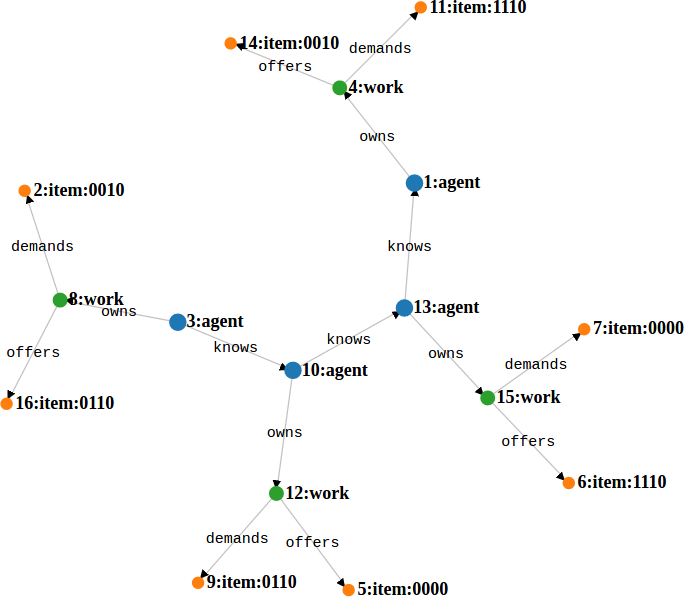
\includegraphics[width=1\textwidth]{toy_graph_before_processes.png}
      \caption{Before similarity search processes, 0 'similarity' links}
      \label{fig:small-before-processes}
    \end{subfigure}
    \begin{subfigure}{0.45\textwidth}
        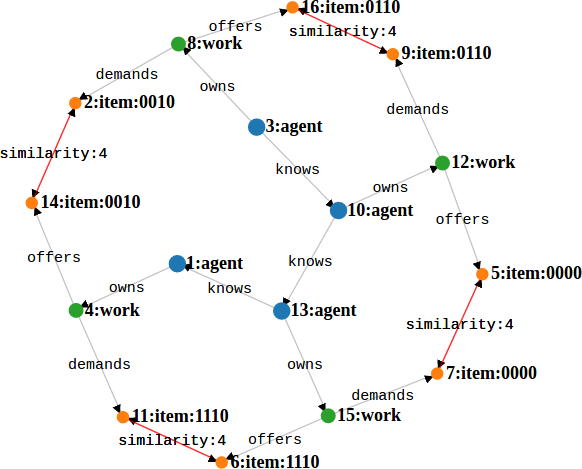
\includegraphics[width=1\textwidth]{toy_graph_after_processes.png}
        \caption{After similarity search processes, 4 'similarity' links forming a cycle}
        \label{fig:small-after-processes}
    \end{subfigure}
    \addtocounter{subfigure}{-1}
    \scriptsize
    \begin{tabular}{ | L{2 cm}  L{0.5 cm} | L{3 cm}  L{0.5 cm} | }
    \hline
    \textbf{Nodes} &  & \textbf{Links} &   \\ \hline
    Agent & 3 & 'knows' & 3  \\ \hline
    Work & 3 & 'owns' & 3 \\ \hline
    Item & 6 & 'demands' / 'offers' & 6 \\ \hline
    \end{tabular}
    \caption{Graph mutations due to similarity search process illustrated on the toy graph.}
    \label{fig:graph-mutations-small-similarity-search}
\end{figure}

\begin{figure}[H]
    \centering
    \captionsetup{justification=centering, size=scriptsize}
    \begin{subfigure}{0.45\textwidth}
        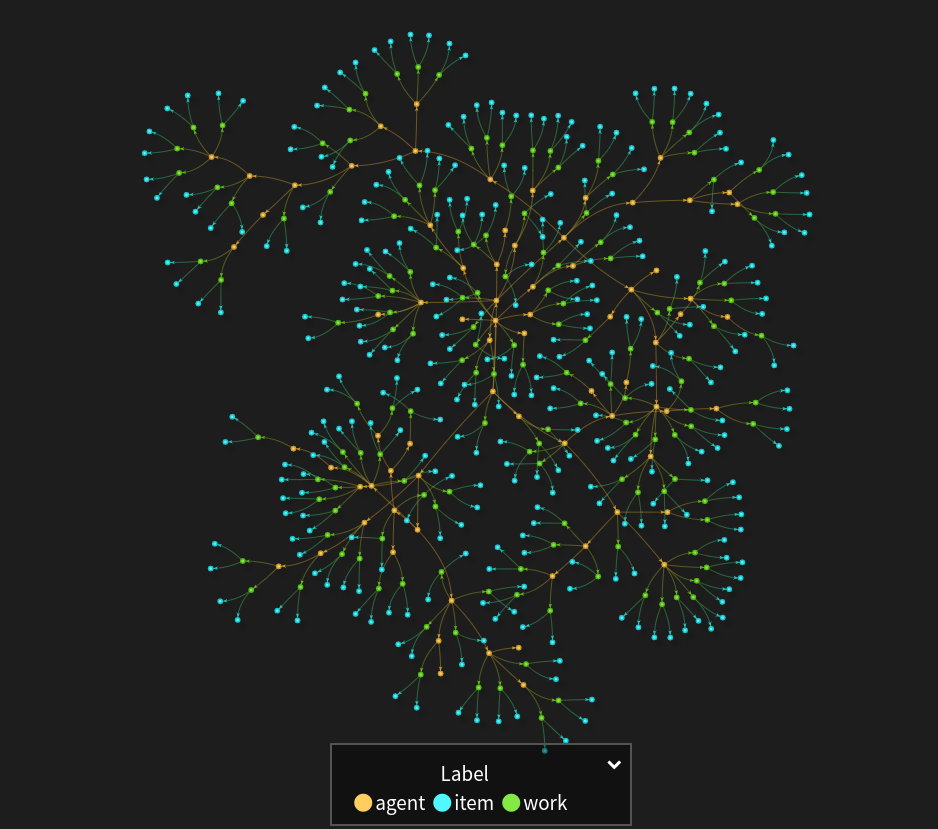
\includegraphics[width=1\textwidth]{larger_graph_before_processing.png}
        \caption{Before similarity search processes, 0 'similarity' links}
        \label{fig:larger-before-processes}
    \end{subfigure}
    \begin{subfigure}{0.45\textwidth}
        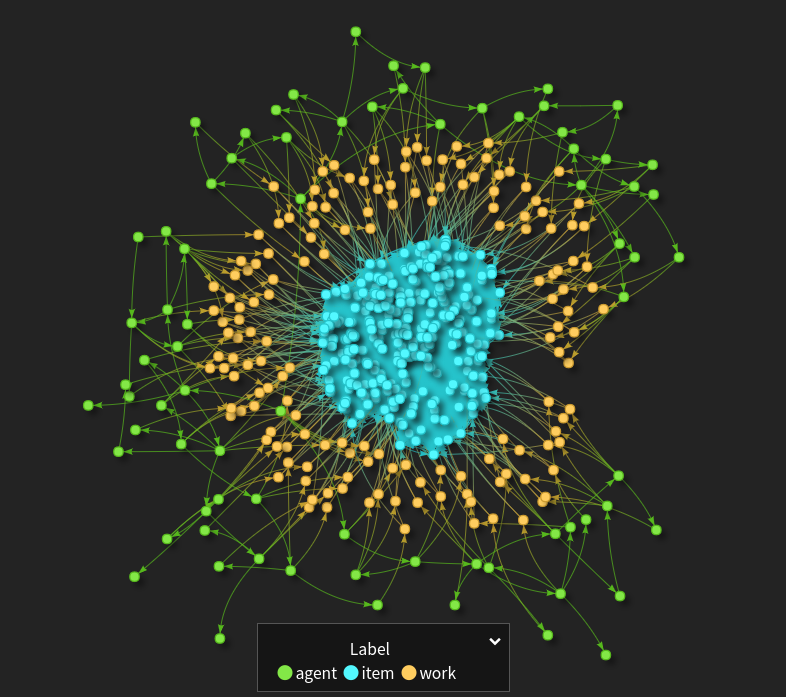
\includegraphics[width=1\textwidth]{larger_graph_after_processing.png}
        \caption{After similarity search processes, 46.574 'similarity' links}
        \label{fig:larger-after-processes}
    \end{subfigure}
    \scriptsize
    \begin{tabular}{ | L{2 cm}  L{0.5 cm} | L{3 cm}  L{0.5 cm} | }
    \hline
    \textbf{Nodes} &  & \textbf{Links} &   \\ \hline
    Agent & 75 & 'knows' & 74  \\ \hline
    Work & 153 & 'owns' & 153 \\ \hline
    Item & 306 & 'demands' / 'offers' & 306 \\ \hline
    \end{tabular}

    \caption{Visualization of larger mutations due to similarity search process.}
    \label{fig:graph-mutations-similarity-search}
\end{figure}


\end{document}